\subsection{Basic word equations}\label{subsec:basiceq}

\newcommand{\pair}[2]{(#1,#2)}

\begin{prop}\label{prop:repstring_origin}
  Let $w$ be a string in $\Sigma^{\ast}$ 
 and $a,b$ constant symbols in $\Sigma$.
  If
  \begin{align}
  wa & = bw, \label{eq:repstring_origin}
  \end{align}
  then $a = b$.
\end{prop}

\begin{proof}
Since it is trivial, we omit the proof.
\end{proof}

\begin{prop}\label{prop:repstring_base}
Let $w$ be a string in $\Sigma^{\ast}$ 
and $a,b,c,d$ constant symbols in $\Sigma$.
If
\begin{align}
wda & = bcw, \label{eq:repstring_base}
\end{align}
then $\pair{b}{c} \in \{\pair{a}{d}, \pair{d}{a}\}$.
\end{prop}

\begin{proof}
  We will prove this proposition by induction on the length of $w$ {\color{red}(i.e., $|w|$)}.
  \begin{itemize}
  \item $|w| = 0,1,2,\mbox{\color{red}~or~}3$: it is straightforward to observe that $\pair{b}{c} \in \{\pair{a}{d}, \pair{d}{a}\}$.
  \item $|w| \ge 4$: We assume that for any string $u$ with $0\leq |u| < n$, if $uda = bcu$, $\pair{b}{c} \in \{\pair{a}{d}, \pair{d}{a}\}$. Since the string $w$ has a prefix $bc$ and a suffix $da$, there exists a string $u$ with $|u| = |w| - 4 < |w|$ such that $w = bcuda$. Since $wda = bcw$, we have $bcudada = bcbcuda$, and then $uda = bcu$. Thus, from the assumption, we get $\pair{b}{c} \in \{\pair{a}{d}, \pair{d}{a}\}$.
  \end{itemize}
From the above, we conclude that if $wda = bcw$, then $\pair{b}{c} \in \{\pair{a}{d}, \pair{d}{a}\}$.
\end{proof}

The conclusion from Proposition~\ref{prop:repstring_base} shows that $\pair{a}{d} \in \{\pair{b}{c}, \pair{c}{b}\}$. Therefore, if $daw = wbc$, we arrive at the same conclusion.

\begin{prop}\label{prop:repstring}
Let $w,w^{\prime}$ be strings of constant symbols in $\Sigma$ and $a,b,c,d$ constant symbols in $\Sigma$.
If
\begin{align}
  wdaw^{\prime} & = w^{\prime}bcw, \label{eq:repstring}
\end{align}
then $\pair{b}{c} \in \{\pair{a}{d}, \pair{d}{a}\}$.\label{prop:repstring_eq}
\end{prop}

\begin{proof}
We will prove this proposition by an induction on $|w| + |w^{\prime}|$.
Without loss of generality, {\color{red} we assume that $|w| \geq |w^{\prime}|$, since the case $|w| < |w^{\prime}|$ similarly leads to} the same conclusion that $\pair{a}{d} \in \{\pair{b}{c}, \pair{c}{b}\}$.
{\color{red}Hence, we have $\pair{b}{c} \in \{\pair{a}{d}, \pair{d}{a}\}$.}
\begin{itemize}
  \item $|w| \geq 0$ and $|w^{\prime}|=0$:
  Eq.~(\ref{eq:repstring}) reduces to $wda = bcw$. By Proposition~\ref{prop:repstring_base}, $\pair{b}{c} \in \{\pair{a}{d}, \pair{d}{a}\}$.
\end{itemize}
We assume that for constant strings $u$ and $u^{\prime}$ with $|u| + |u^{\prime}| < |w| + |w^{\prime}|$, if $udau^{\prime} = u^{\prime}bcu$, then $\pair{b}{c} \in \{\pair{a}{d}, \pair{d}{a}\}$.
We divide the relations between $|w|$ and $|w^{\prime}|$ into the following four cases:
\begin{itemize}
\item $0 < |w^{\prime}| \le |w| \le |w^{\prime}|+1$:
When either $|w|=|w^{\prime}|$ or $|w|=|w^{\prime}|+1$, Eq.~(\ref{eq:repstring}) is illustrated in Figs.~\ref{fig:prop_pic7} and \ref{fig:prop_pic8}, respectively.
If $|w|=|w^{\prime}|$, $\pair{b}{c} = \pair{d}{a}$.
If $|w|=|w^{\prime}|+1$, $d = c$ and $w = w^{\prime}b = aw^{\prime}$.
From Proposition~\ref{prop:repstring_origin}, we deduce that $b = a$.
Therefore, $\pair{b}{c} \in \{\pair{a}{d}, \pair{d}{a}\}$.
%
\item $|w^{\prime}|+2 \le |w| \le 2|w^{\prime}| - 1$:
In Eq.~\ref{eq:repstring}, since $|wdaw^{\prime}| = |w^{\prime}bcw| = |w| + |w^{\prime}| + 2$, a suffix of $w$ overlaps with a prefix of $w$, as illustrated in Fig.~\ref{fig:prop_pic9}.
That is, there exists a constant string $u$ of length $2|w| - (|w| + |w^{\prime}| + 2) = |w| - |w^{\prime}| - 2$ such that $u$ is both a prefix and a suffix of $w$.
Since $uda$ has a length of $|w| - |w^{\prime}|$, it is also a prefix of $w$. Similarly, $bcu$ is a suffix of $w$.
Because {\color{red}$|w| - (|uda| + |bcu|) = 2|w^{\prime}| - |w| \ge 1$}, there exists a constant string $u^{\prime}$ of length $2|w^{\prime}| - |w|$ such that $w = udau^{\prime}bcu$.
Since $w^{\prime}$ is a suffix of $w$ and $|u^{\prime}bcu| = (2|w^{\prime}| - |w|) + 2 + (|w| - |w^{\prime}| - 2) = |w^{\prime}|$, we have $w^{\prime} = u^{\prime}bcu$.
Similarly, $w^{\prime} = udau^{\prime}$. Thus, we derive the equation $u^{\prime}bcu = udau^{\prime}$.
Since $|u| = |w| - |w^{\prime}| - 2 \leq |w| - 3 < |w|$ and $|u^{\prime}| = 2|w^{\prime}| - |w| < |w^{\prime}|$, i.e., $|u| + |u^{\prime}| < |w| + |w^{\prime}|$, the induction hypothesis on $|u| + |u^{\prime}|$ implies that $\pair{b}{c} \in \{\pair{a}{d}, \pair{d}{a}\}$.
%
\item $2|w^{\prime}| \le |w| \le 2|w^{\prime}|+3$:
When $|w|=2|w^{\prime}|$, it is straightforward to observe that $w = w^{\prime}w^{\prime}$.
Therefore, $w^{\prime}da = bcw^{\prime}$, as illustrated in Fig.~\ref{fig:prop_pic14}.
From Proposition~\ref{prop:repstring_base}, $\pair{b}{c} \in \{\pair{a}{d}, \pair{d}{a}\}$.
When $|w|=2|w^{\prime}|+i$ ($i=1,2,3$), Eq.~(\ref{eq:repstring}) is depicted in Figs.~\ref{fig:prop_pic13}, \ref{fig:prop_pic12}, and \ref{fig:prop_pic11}, respectively.
When $|w|=2|w^{\prime}|+2$, it is clear that $\pair{b}{c} = \pair{d}{a}$. 
When $|w|=2|w^{\prime}|+1$ and $|w|=2|w^{\prime}|+3$, Proposition~\ref{prop:repstring_origin} implies that $\pair{b}{c} = \pair{a}{d}$.
%
\item $2|w^{\prime}|+4 \leq |w|$:
Since the strings $w^{\prime}bc$ and $adw^{\prime}$ are a prefix and a suffix of $w$, respectively, and $|w^{\prime}bc| + |adw^{\prime}| = 2|w^{\prime}| + 4$, there exists a string $u$ with $|u| \geq 0$ such that $w = w^{\prime}bcudaw^{\prime}$.
From Eq.~(\ref{eq:repstring}), $w^{\prime}bcudaw^{\prime}daw^{\prime} = w^{\prime}bcw^{\prime}bcudaw^{\prime}$, i.e., $udaw^{\prime} = w^{\prime}bcu$, as illustrated in Fig.~\ref{fig:prop_pic10}.
Let $u^{\prime} = w^{\prime}$.
Since $|u| + |u^{\prime}| = |w|- (2|w^{\prime}| + 4) + |w^{\prime}| < |w| + |w^{\prime}|$, the induction hypothesis on $|u| + |u^{\prime}|$ implies that $\pair{b}{c} \in \{\pair{a}{d}, \pair{d}{a}\}$.
\end{itemize}
From the above, we conclude that if $wdaw^{\prime} = w^{\prime}bcw$, then $\pair{b}{c} \in \{\pair{a}{d}, \pair{d}{a}\}$.
\end{proof}

\begin{figure}[t]
\begin{center}
  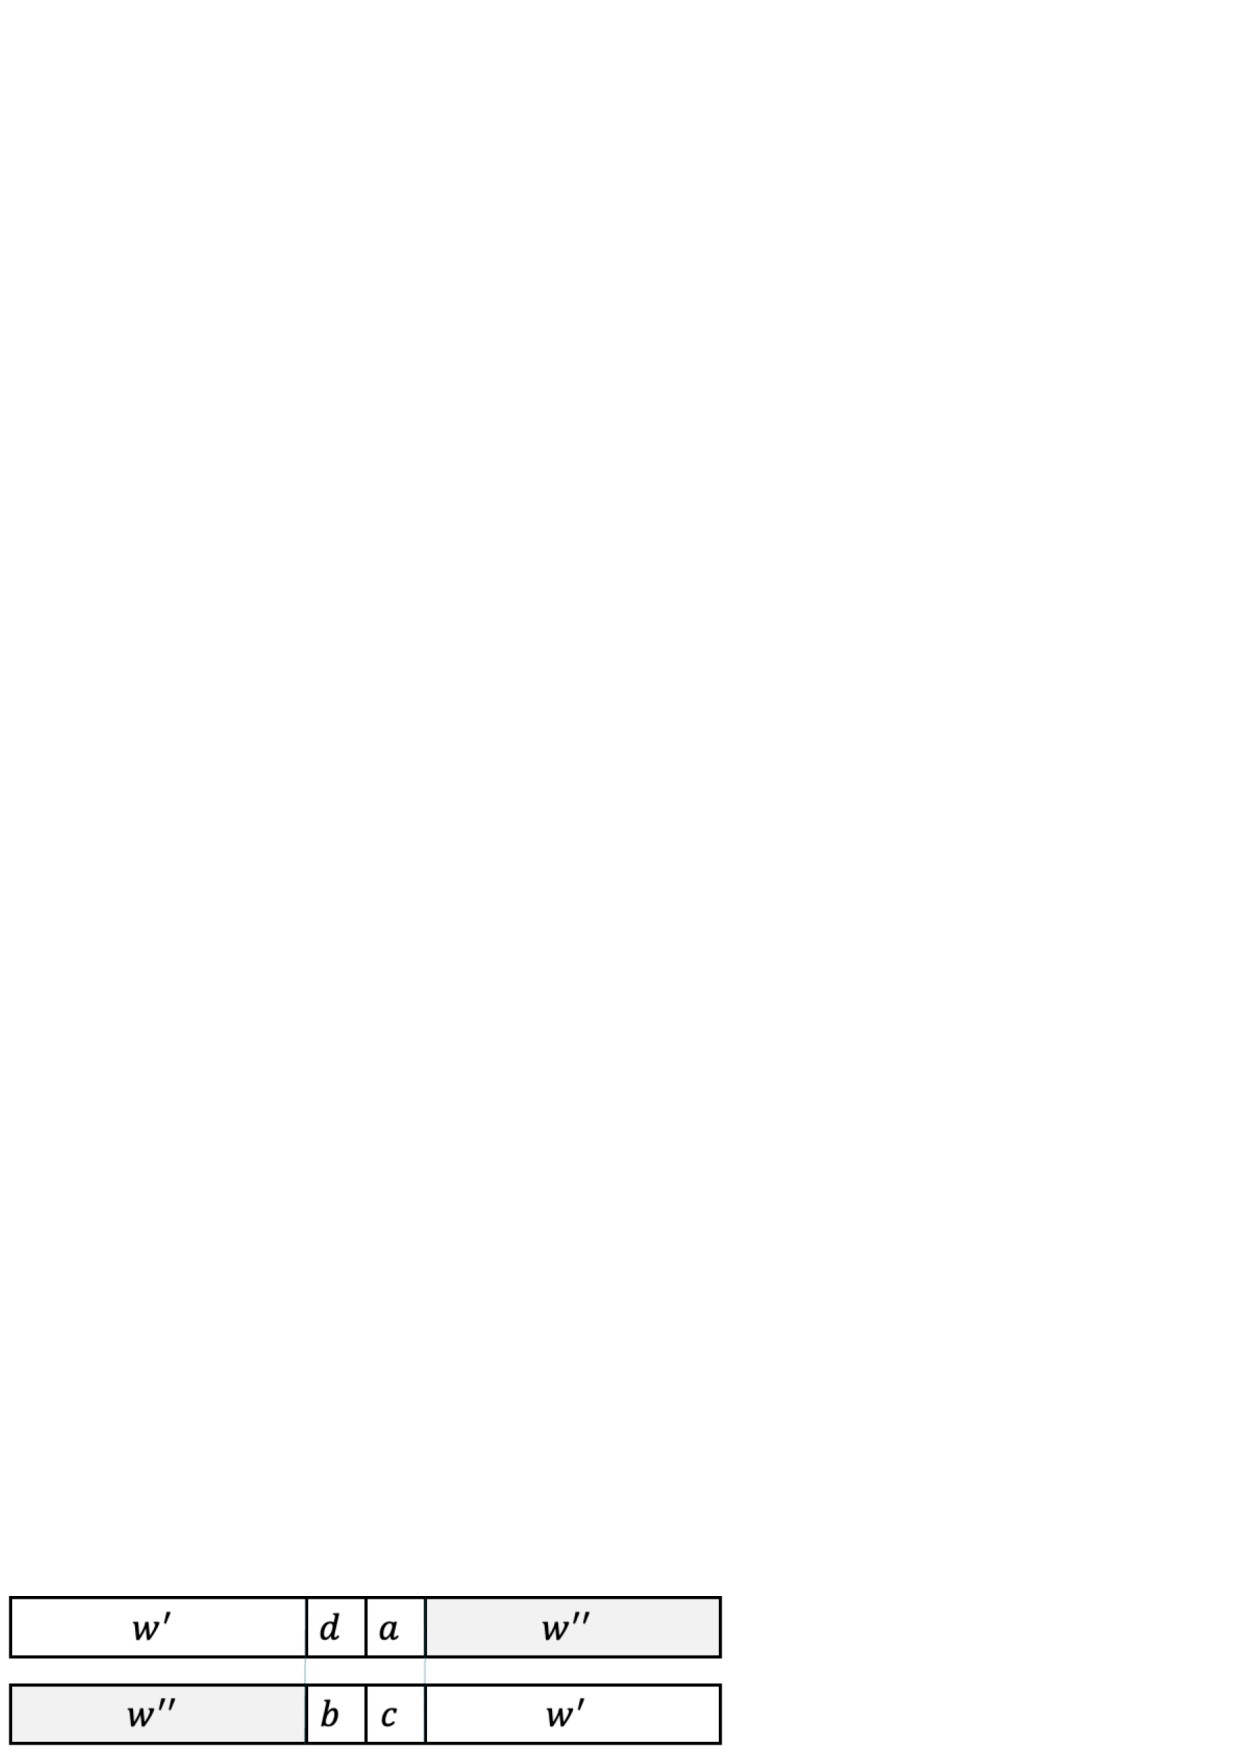
\includegraphics[scale=0.345]{figs/w=w_1.pdf}
  \caption{Case $|w| = |w^{\prime}|$ in Proposition~\ref{prop:repstring}}\label{fig:prop_pic7}
  \bigskip
  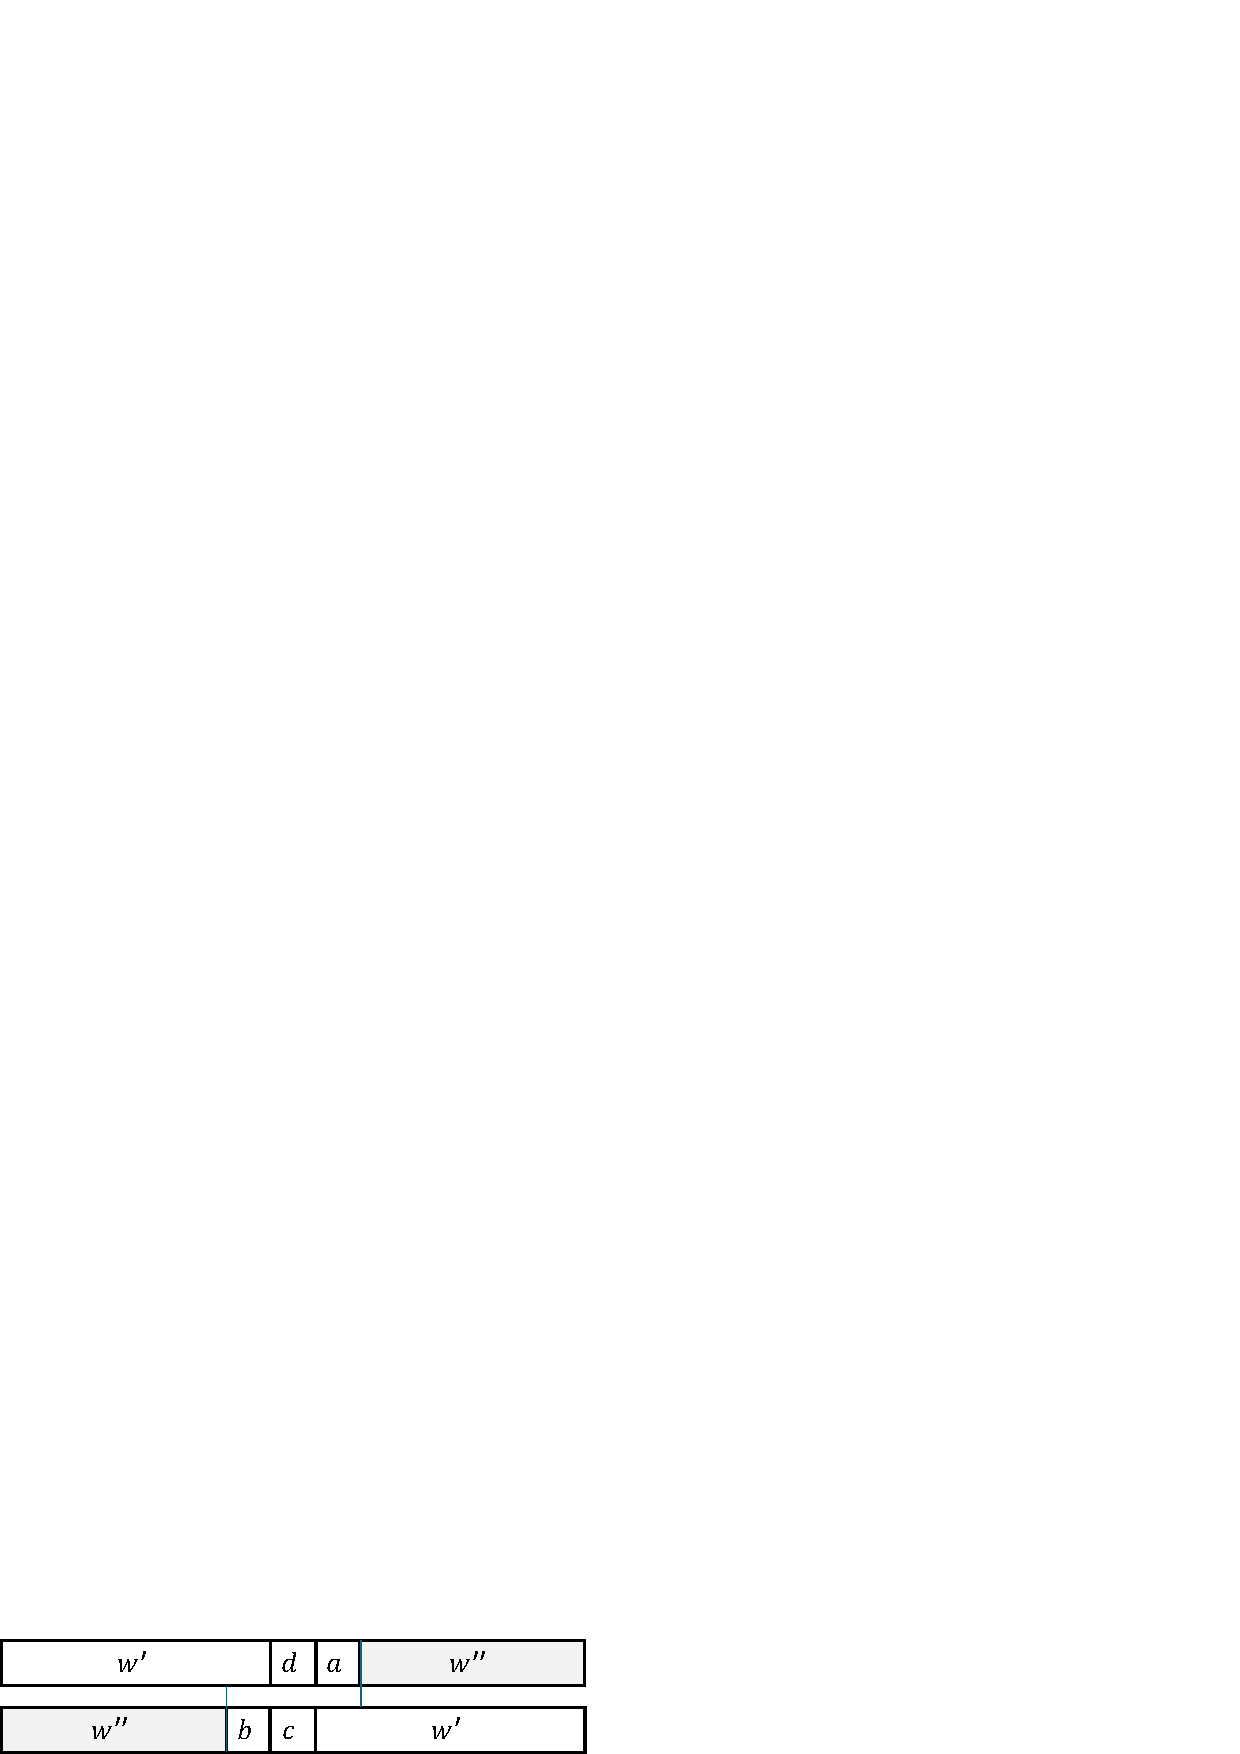
\includegraphics[scale=0.345]{figs/w=w_1+1.pdf}
  \caption{Case $|w| = |w^{\prime}| + 1$ in Proposition~\ref{prop:repstring}}\label{fig:prop_pic8}
\end{center}
\end{figure}

\begin{figure}[t]
\begin{center}
  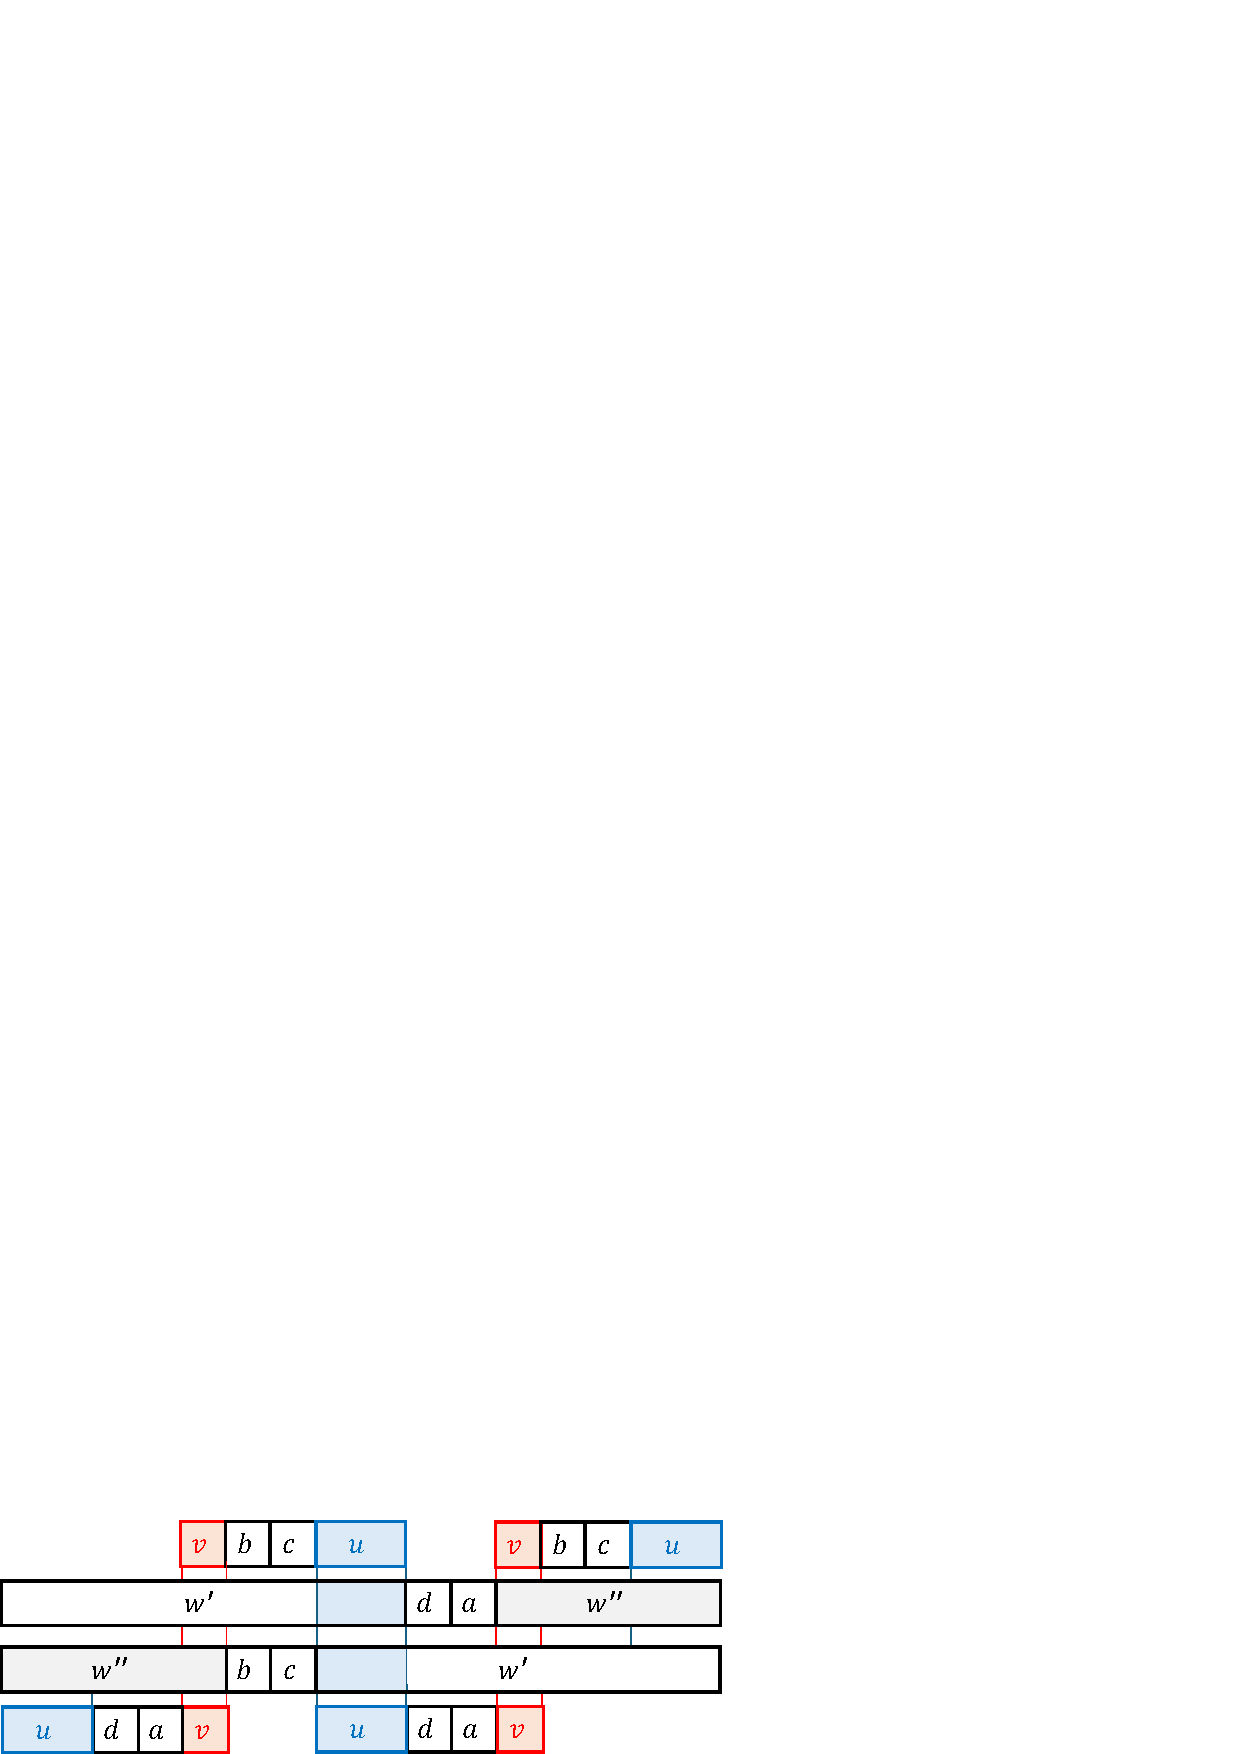
\includegraphics[scale=0.345]{figs/w=w_1+2.pdf}
  \caption{Case $|w^{\prime}| + 2 \le |w| \le 2|w^{\prime}| - 1$ in Proposition~\ref{prop:repstring}}\label{fig:prop_pic9}
\end{center}
\end{figure}

\begin{figure}[t]
\begin{center}
  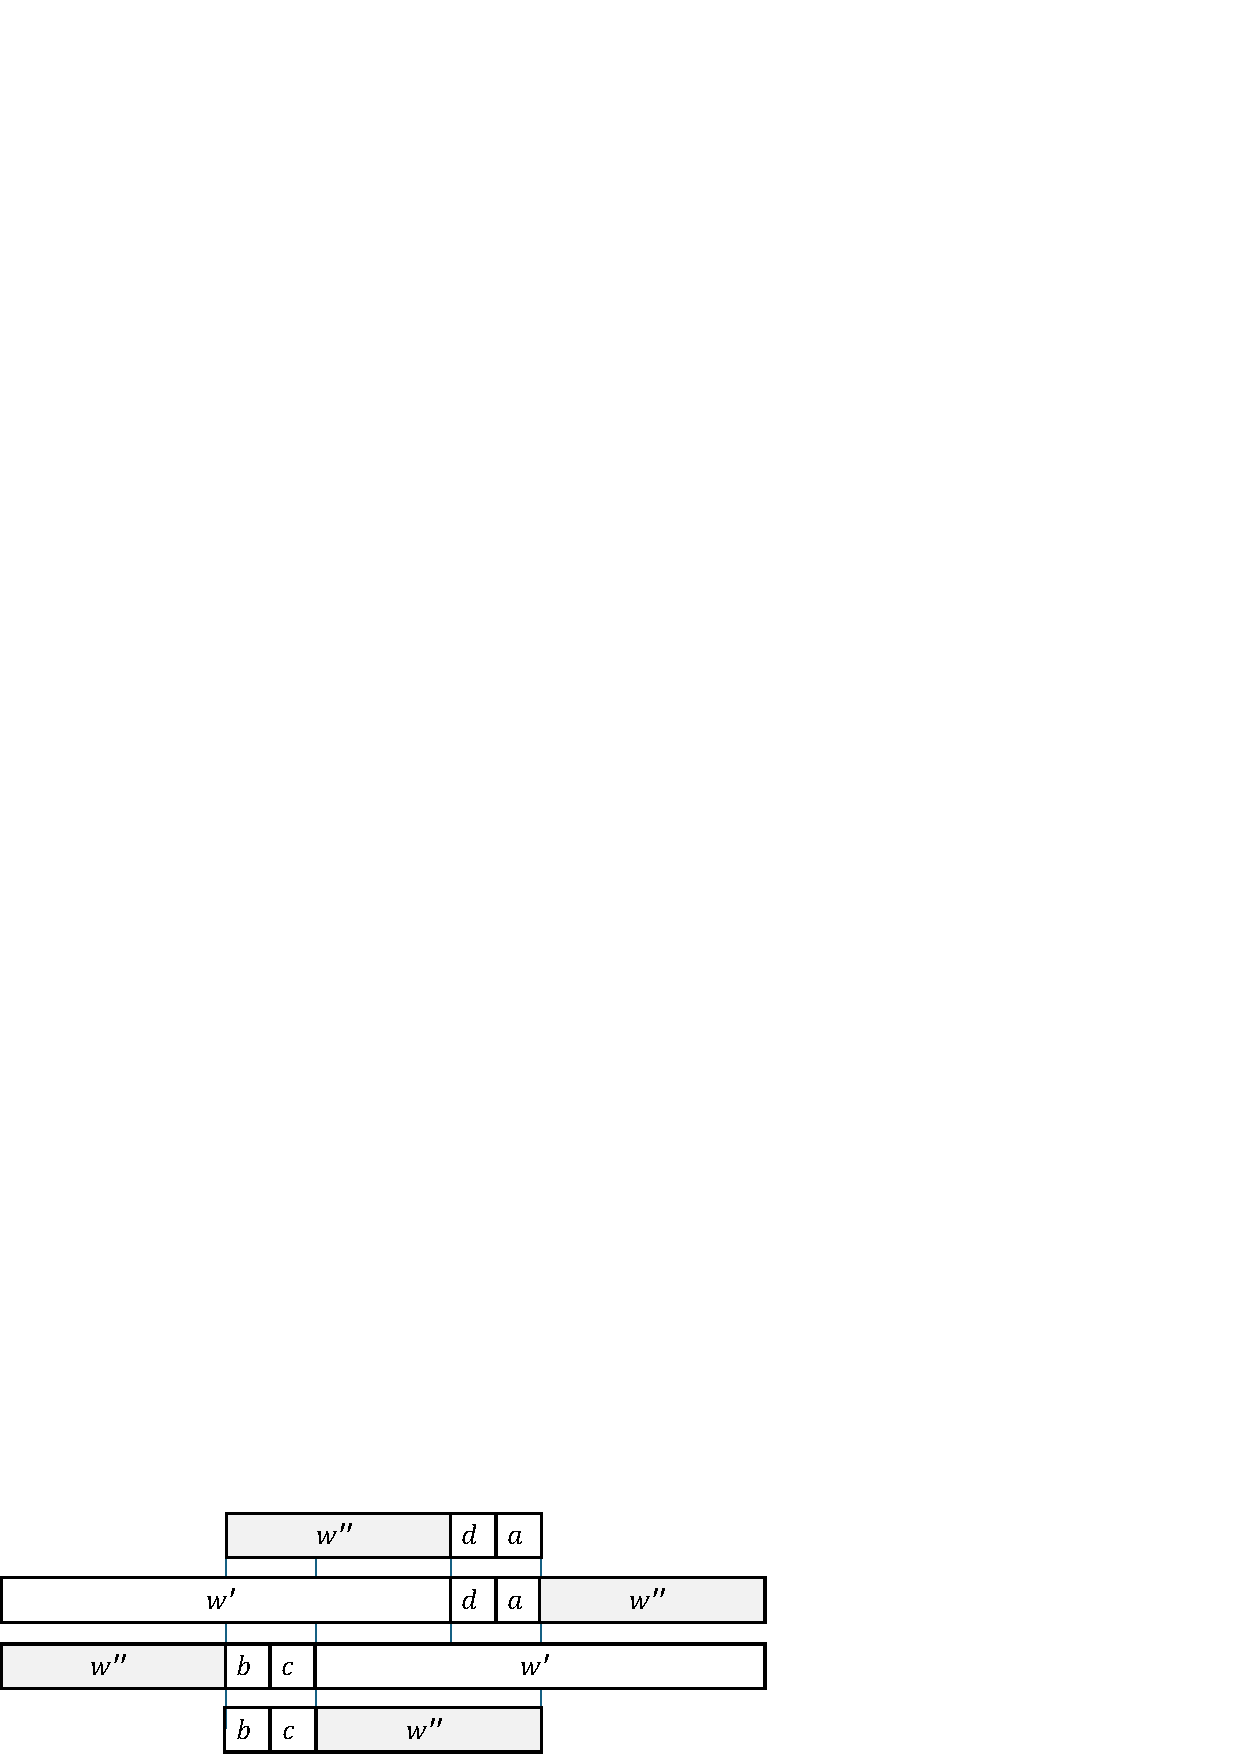
\includegraphics[scale=0.345]{figs/w=2w_1.pdf}
  \caption{Case $|w| = 2|w^{\prime}|$ in Proposition~\ref{prop:repstring}}\label{fig:prop_pic14}
  \bigskip
  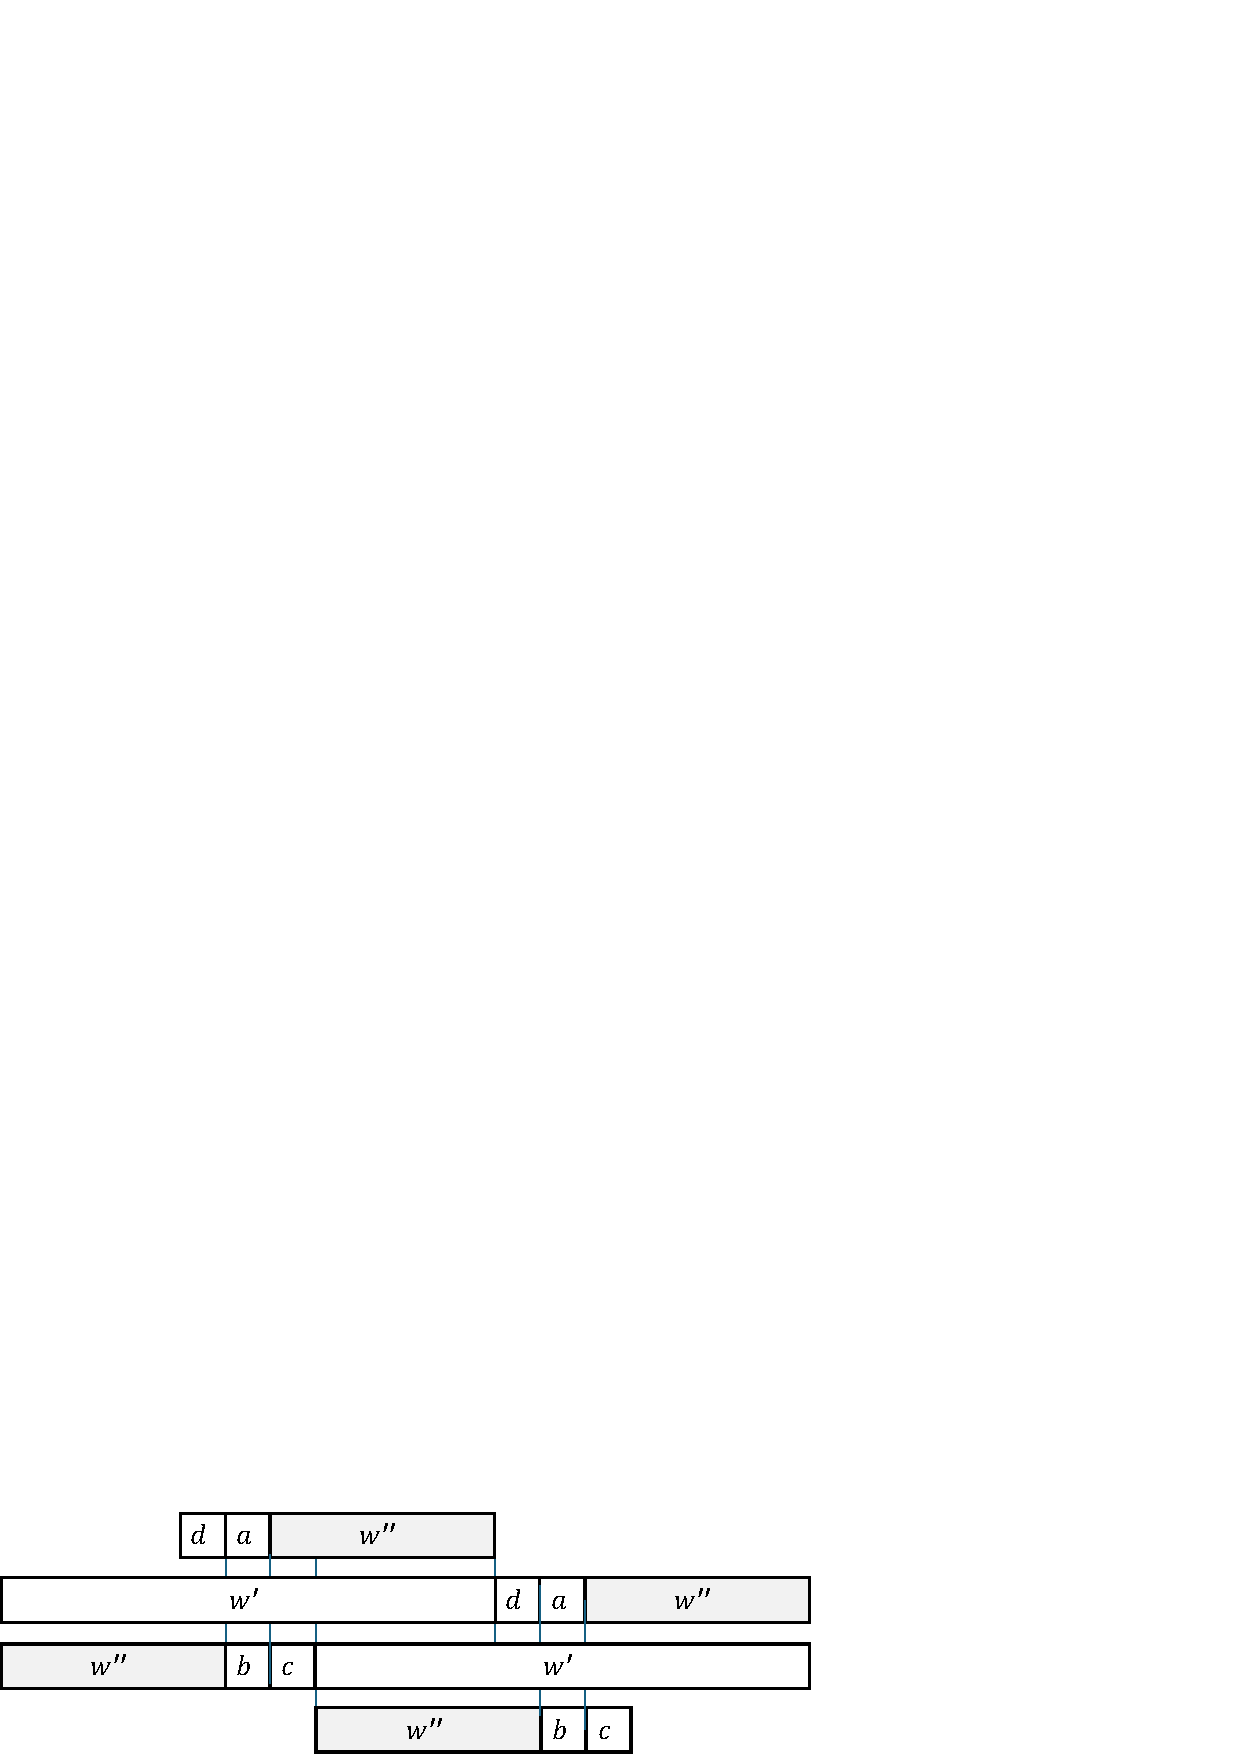
\includegraphics[scale=0.345]{figs/w=2w_1+1.pdf}
  \caption{Case $|w| = 2|w^{\prime}| + 1$ in Proposition~\ref{prop:repstring}}\label{fig:prop_pic13}
  \bigskip
  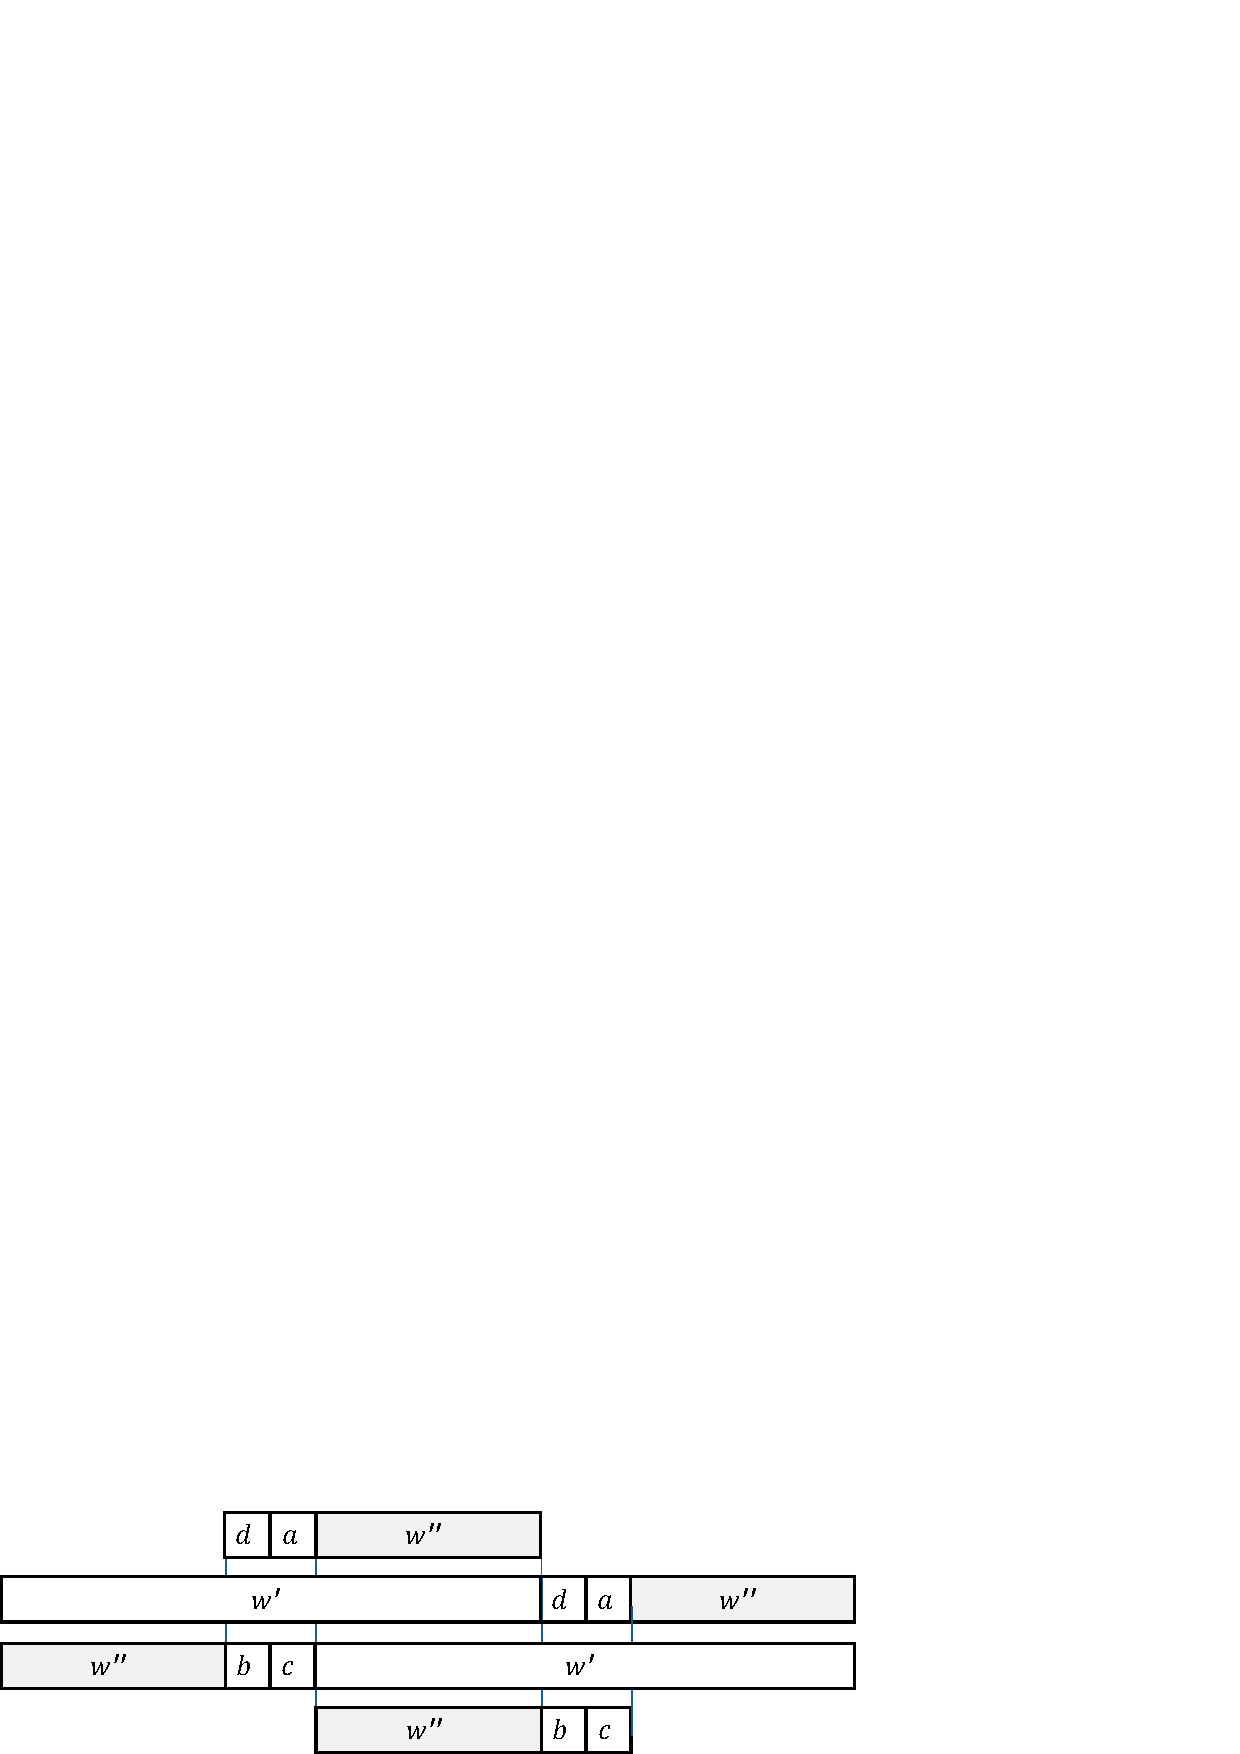
\includegraphics[scale=0.345]{figs/w=2w_1+2.pdf}
  \caption{Case $|w| = 2|w^{\prime}| + 2$ in Proposition~\ref{prop:repstring}}\label{fig:prop_pic12}
  \bigskip
  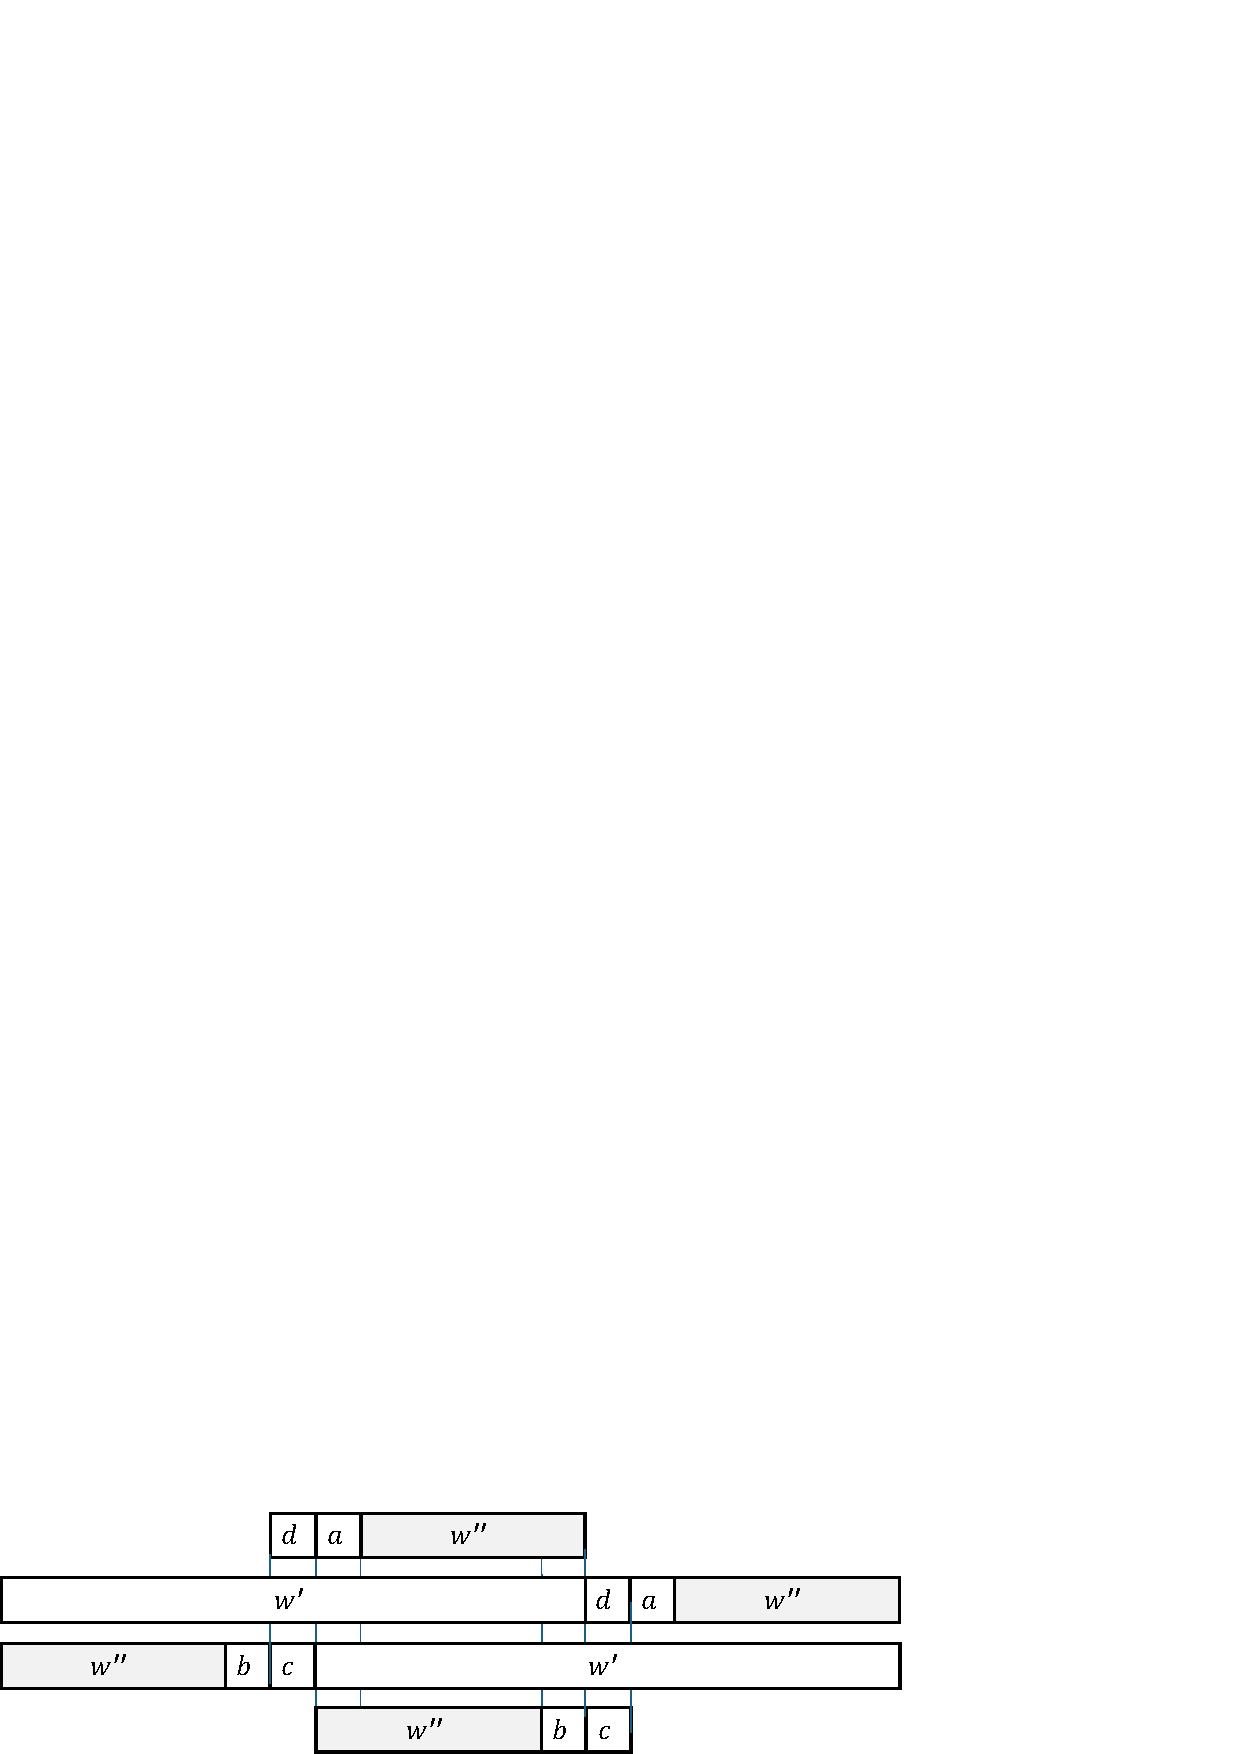
\includegraphics[scale=0.345]{figs/w=2w_1+3.pdf}
  \caption{Case $|w| = 2|w^{\prime}| + 3$ in Proposition~\ref{prop:repstring}}\label{fig:prop_pic11}
\end{center}
\end{figure}

\begin{figure}[t]
\begin{center}
  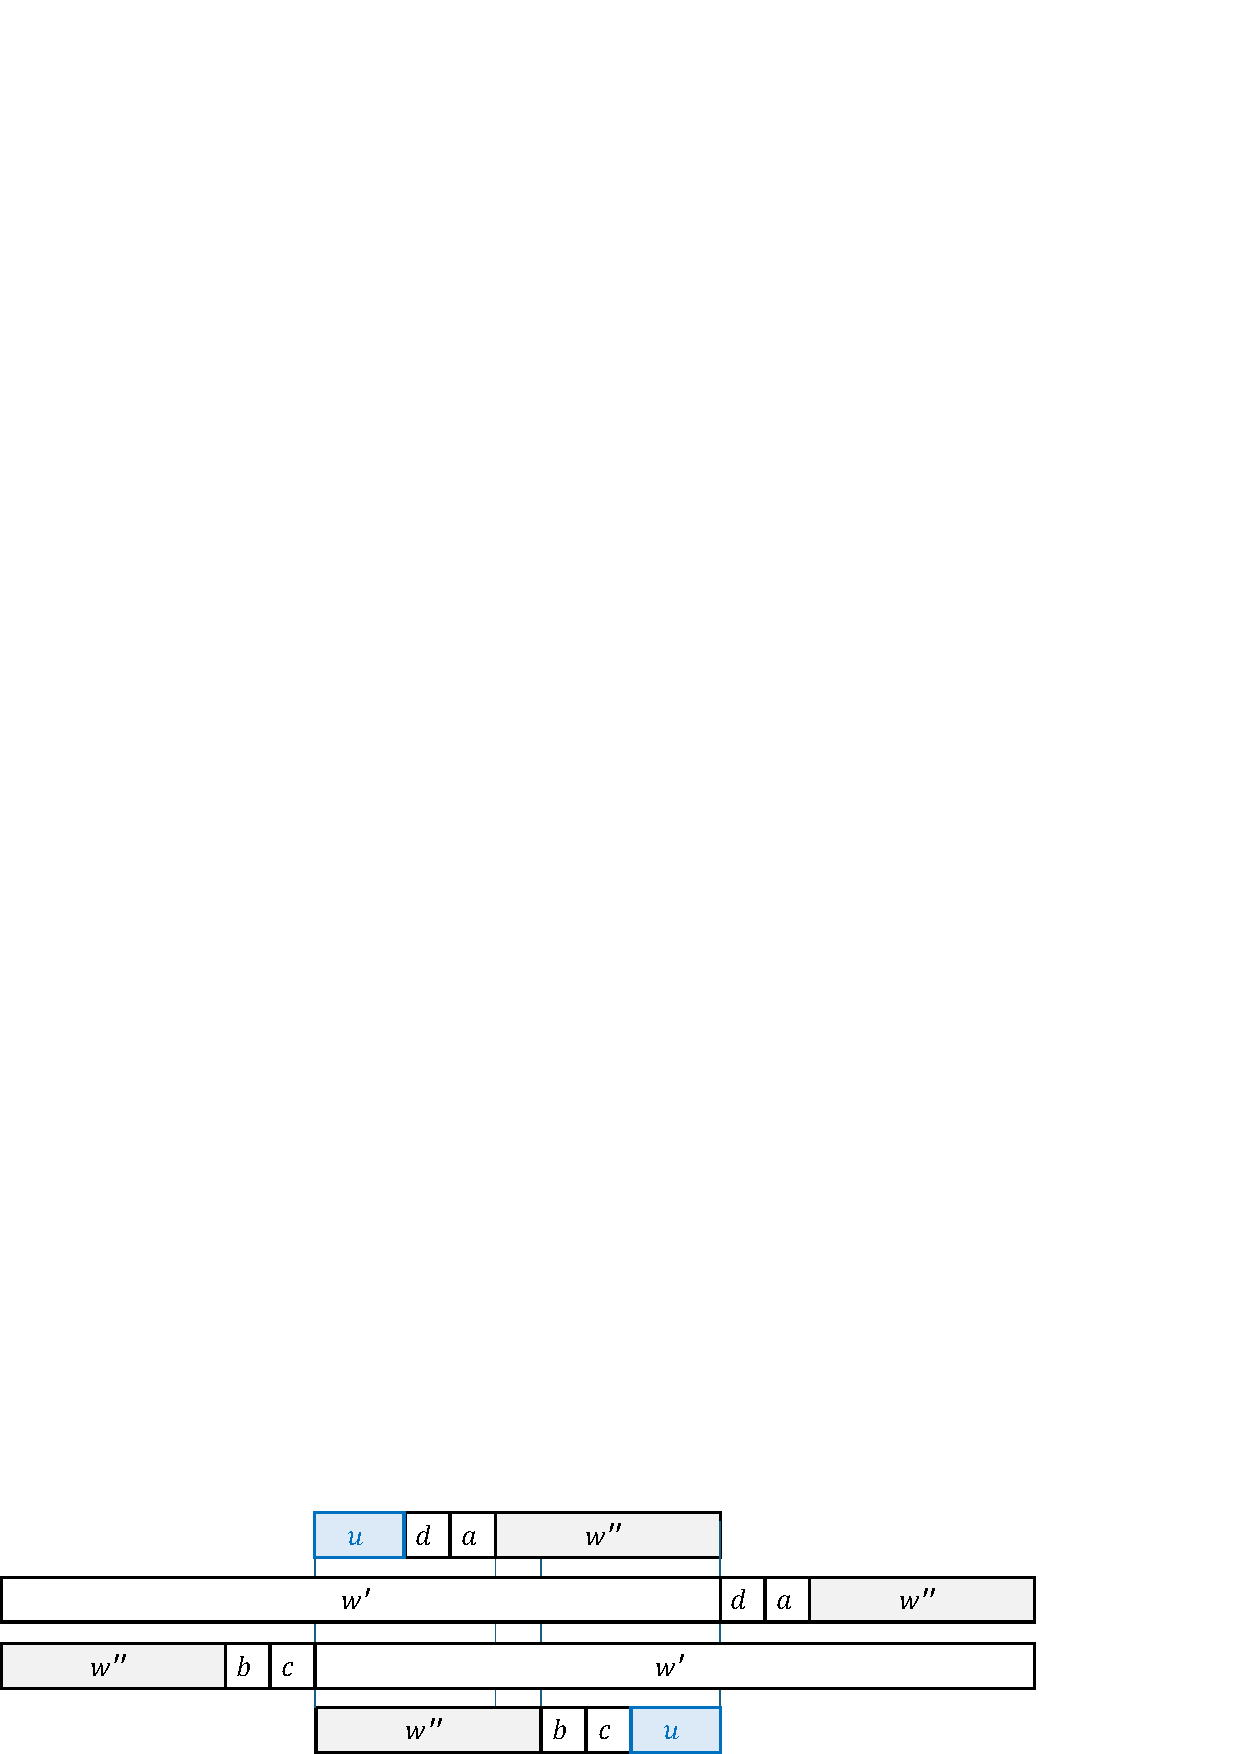
\includegraphics[scale=0.345]{figs/w=2w_1+4.pdf}
  \caption{Case $2|w^{\prime}| + 4 \leq |w|$ in Proposition~\ref{prop:repstring}}\label{fig:prop_pic10}
\end{center}
\end{figure}